\documentclass{article}

\usepackage{graphicx}
\usepackage{tikz}
\usepackage{tikzsymbols}
\usetikzlibrary{calc,patterns,shapes.geometric}
\pagestyle{empty}
\usepackage[margin=0pt]{geometry}
\geometry{papersize={14in,12in}}

\def\centerarc[#1](#2)(#3:#4:#5){\draw[#1] ($(#2)+({#5*cos(#3)},{#5*sin(#3)})$) arc (#3:#4:#5);}

\begin{document}
	\begin{figure}
		\centering
		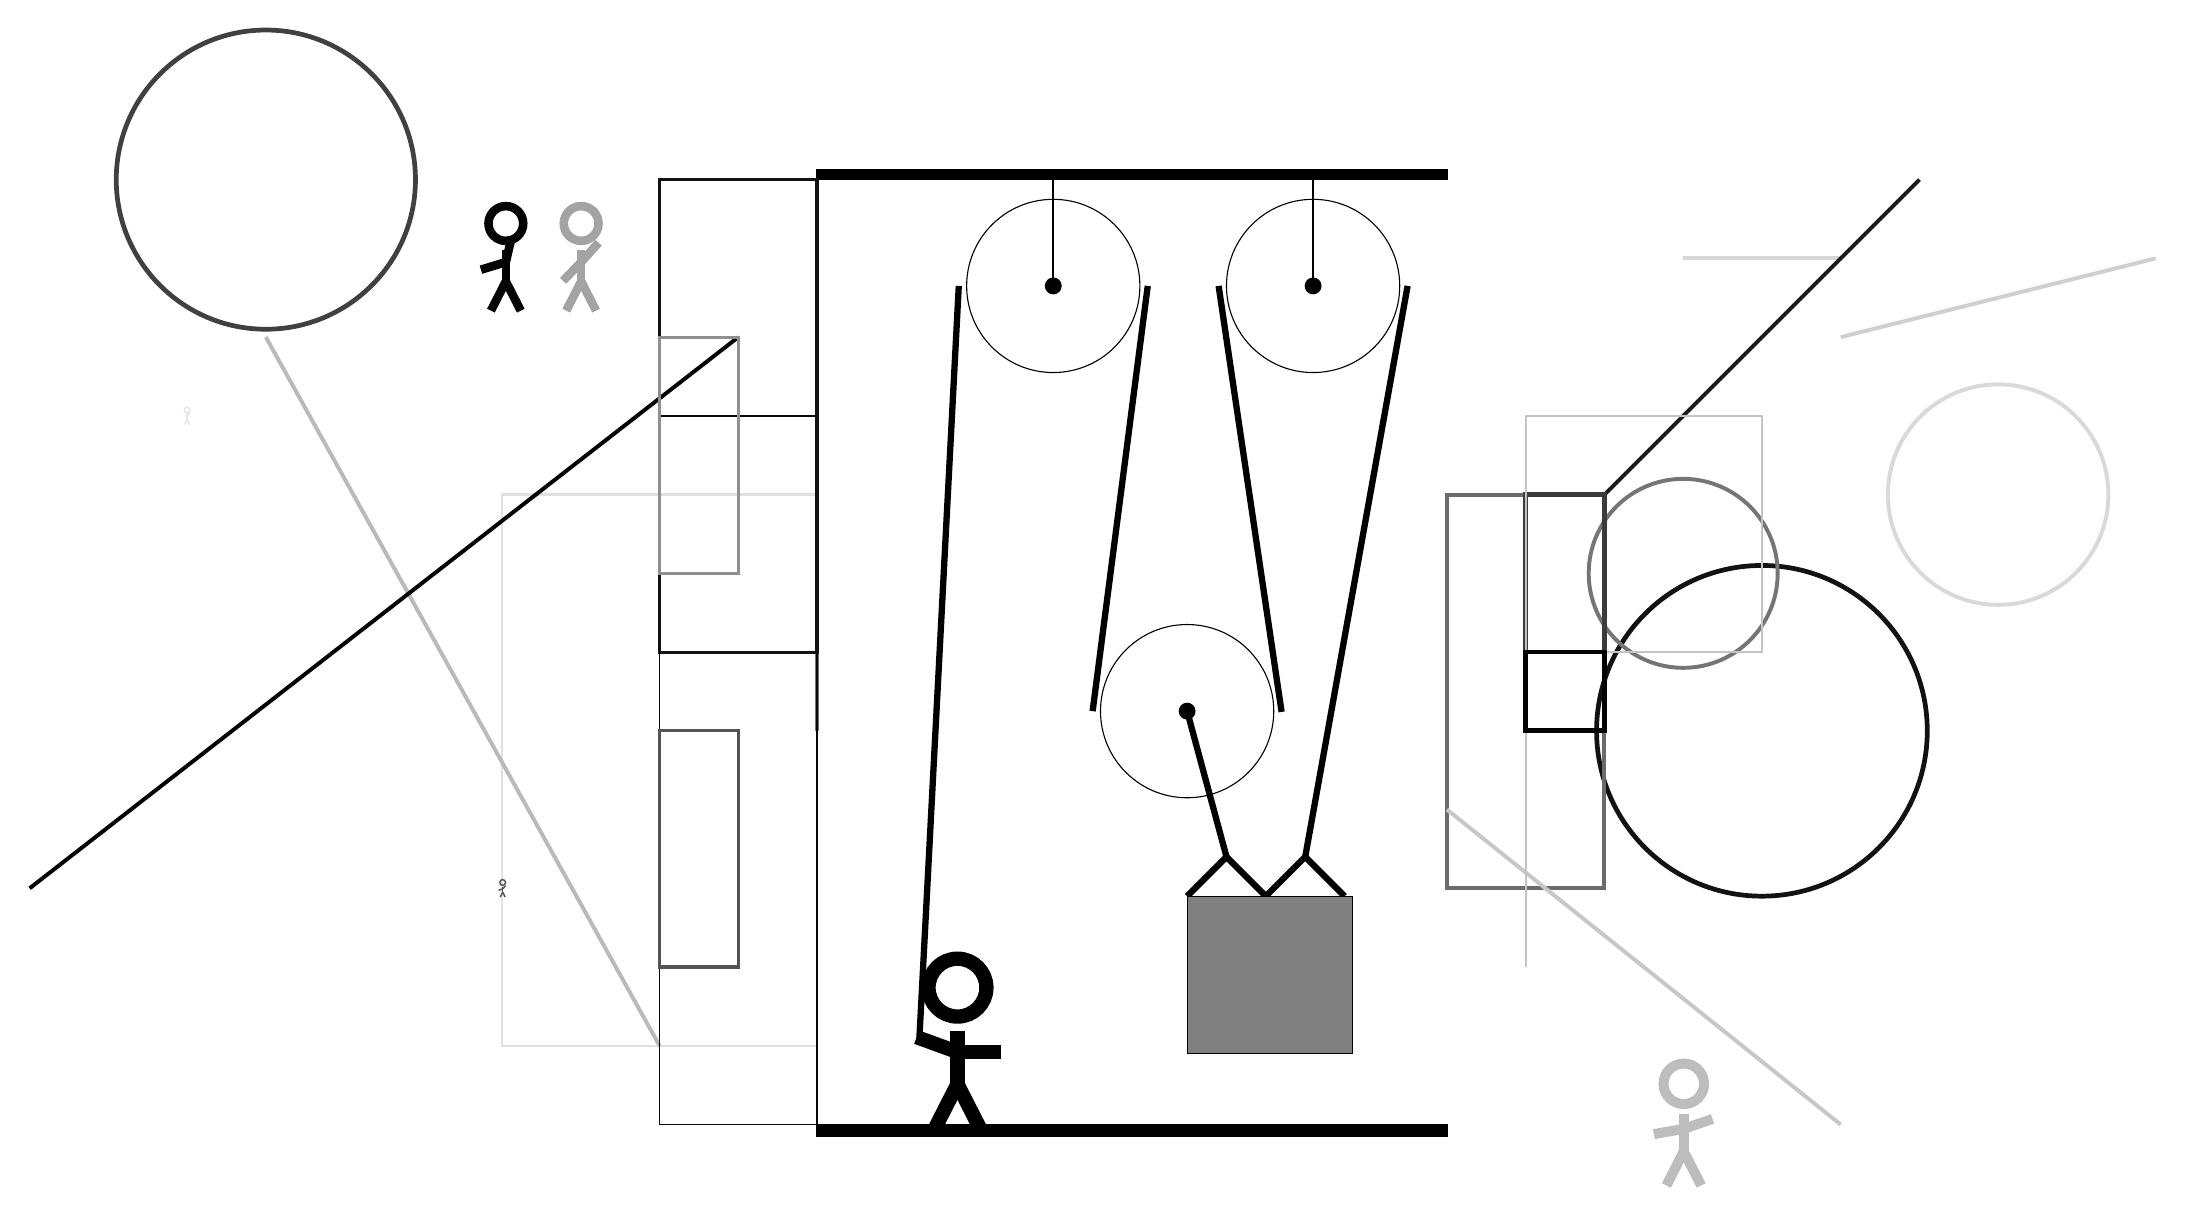
\begin{tikzpicture}
			%%%%% START %%%%%
			
			\draw[fill=black] (-2, 9) rectangle (6, 9.125);
			
			\draw (1, 7.65) circle (1.1);
			\draw[fill=black] (1, 7.65) circle (0.1);
			\draw[thick] (1, 7.65) -- (1, 9);
			
			\draw (4.3, 7.65) circle (1.1);
			\draw[fill=black] (4.3, 7.65) circle (0.1);
			\draw[thick] (4.3, 7.65) -- (4.3, 9);
			
			\draw (2.7, 2.25) circle (1.1);
			\draw[fill=black] (2.7, 2.25) circle (0.1);
			
			\draw[line width=0.8mm]  (2.7, -0.1) -- (3.2, 0.4) -- (3.7, -0.1) -- (4.2, 0.4) -- (4.7, -0.1);
			\draw[fill=black!50] (2.7, -0.1) rectangle (4.8, -2.1);
			
			\draw[line width=0.8mm](-0.7, -1.9) -- (-0.2, 7.65);
			\centerarc[line width=0.8mm](1, 7.65)(0:180:1.2000000000000002);
			\draw[line width=0.8mm](2.2, 7.65) -- (1.5, 2.25);
			\centerarc[line width=0.8mm](2.7, 2.25)(180:370:1.2000000000000002);
			\draw[line width=0.8mm] (3.9, 2.24) -- (3.1, 7.65);
			\centerarc[line width=0.8mm](4.3, 7.65)(0:180:1.2000000000000002);
			\draw[line width=0.8mm](4.2, 0.4) -- (5.5, 7.65);
			\draw[line width=0.8mm] (3.2, 0.4) -- (2.7, 2.25);
			
			\node at (-0.2, -2) {\Strichmaxerl[10][-20][0]};
			
			\draw[line width=0.3mm, color=black!12] (-2, -2) rectangle (-6, 5);
			
			\draw [line width=0.6mm, color=black!93](10, 2) circle (2.1);
			\node[line width=0.3mm, color=black!99] at (-6, 8) {\Strichmaxerl[6][17][77]};
			\draw[line width=0.5mm, color=black!27](-4, -2) -- (-9, 7);
			\draw [line width=0.5mm, color=black!54](9, 4) circle (1.2);
			\draw[line width=0.5mm, color=black!58] (8, 0) rectangle (6, 5);
			
			\node[line width=0.7mm, color=black!36] at (-5, 8) {\Strichmaxerl[6][46][48]};
			
			\draw[line width=0.5mm, color=black!54](-2, 3) -- (-2, 2);
			\draw[line width=0.5mm, color=black!16](9, 8) -- (11, 8);
			\draw[line width=0.5mm, color=black!89](8, 5) -- (12, 9);
			\draw[line width=0.2mm, color=black!97] (-4, -3) rectangle (-2, 6);
			\draw[line width=0.5mm, color=black!88](-2, 9) -- (-2, 5);
			\draw[line width=0.6mm, color=black!77] (8, 2) rectangle (7, 5);
			
			\node[line width=0.2mm, color=black!10] at (-10, 6) {\Strichmaxerl[1][85][62]};
			\draw [line width=0.6mm, color=black!75](-9, 9) circle (1.9);
			\draw[line width=0.3mm, color=black!23] (7, 3) rectangle (10, 6);
			
			\draw[line width=0.5mm, color=black!22](11, -3) -- (6, 1);
			
			\node[line width=0.7mm, color=black!67] at (-6, 0) {\Strichmaxerl[1][18][47]};
			\draw[line width=0.5mm, color=black!19](11, 7) -- (15, 8);
			\draw[line width=0.4mm, color=black!67] (-3, -1) rectangle (-4, 2);
			\draw[line width=0.3mm, color=black!24] (7, -1) rectangle (7, 4);
			
			\draw[line width=0.5mm, color=black!99](-3, 7) -- (-12, 0);
			\draw[line width=0.6mm, color=black!99] (7, 2) rectangle (8, 3);
			\node[line width=0.4mm, color=black!26] at (9, -3) {\Strichmaxerl[7][10][19]};
			\draw [line width=0.5mm, color=black!15](13, 5) circle (1.4);
			
			\draw[line width=0.4mm, color=black!93] (-4, 3) rectangle (-2, 9);
			\draw[line width=0.4mm, color=black!44] (-4, 4) rectangle (-3, 7);
			
			\draw[fill=black] (-2, -3) rectangle (6, -3.15);
			
			%%%%% END %%%%%
		\end{tikzpicture}
	\end{figure}	
\end{document}